\documentclass[a4paper ,12pt, onecolumn]{article}
\usepackage[utf8]{inputenc}
\usepackage[spanish]{babel}

\usepackage[hidelinks]{hyperref}
\usepackage{graphicx}
\graphicspath{ {./images/} }


\begin{document}

\title{Sistemas de posicionamiento de objetos mediante tecnología Bluetooth Low Energy
Beacon }
\author{Rubén Arce}
\date{\today}
\maketitle
\cleardoublepage
\tableofcontents
\cleardoublepage
\section{Memoria descriptiva}
Antecedentes, objeto, normativa, reglamentación
Extensión máxima de 30 páginas + anexos 60
Defensa de 20 min  40
    \subsection{Antecedentes y objeto del proyecto}
        Este proyecto surge como solución a una necesidad de poder localizar un número elevado de equipos en 
        constante movimiento con cierta exactitud en un espacio cerrado.
        \begin{enumerate}
            \item Estudio sobre las distintas alternativas para llevar a cabo este tracking de objetos de una forma
            sencilla y sin requerir de una inversión grande.
            \item Análisis de las tecnologías existentes para la monitorización en interiores.
            \item  Estudio del parámetro RSSI como medida de la potencia de una señal y cálculo de la distancia entre equipos.
            \item Desarrollo de un sistema de visualización mediante un mapa sobre el que poder ver los equipos en movimiento.
            \item Diseño de hardware específico para la aplicación requerida.
            \item Programación tanto del equipo emisor como del receptor así como del algoritmo de visualización.
            \item Pruebas de campo y comprobación del rendimiento del equipo.
        \end{enumerate}
    \subsection{Ambito de aplicación}
        El tracking de objetos en espacios cerrados está día a día incrementando su popularidad debido a que es una 
        arma de propaganda muy poderosa que demandan los grandes hipermercados para llevar a cabo estudios de marketing
        y poder analizar el comportamiento de los clietes.
        \paragraph{}
        Los principales ámbitos de aplicación de esta tecnología son:
        \begin{enumerate}
            \item Marketing: Estudios de mercado y de necesidad de los clientes. "heat map"
            \item Seguridad: Tan solo los empleados con autorización y proximidad podrán llevar a cabo acciones.
            \item Vandalismo: Conociendo la localización de los equipos dentro de un local cerrado en el momento 
            en el que se deja de situar un elemento se puede dar la voz de alarma ante un robo.
            \item Anuncios y nueva forma de publicidad: Activar acciones en función de la localización en determinados puntos de interés
        \end{enumerate}
    \subsection{Análisis de soluciones}
        \subsubsection {Wifi}
        Consume como un demonio, inviable 
        \subsubsection {GPS}
        A diferencia de la tecnología GPS, tiene potencial como sistema de posicionamiento en interiores y su consumo de batería es muy reducido.

        \subsubsection {Bluetooth Low Energy}
        Existen varios tipos de beacons:
        https://accent-systems.com/es/producto/ibks-105/
        \begin{enumerate}
            \item iBeacon: Fue la primera tecnología BLE Beacon desarrollada por Apple, permite leer y emitir en modo 
            broadcast para cualquier dispositivo que disponga de Bluetooth low energy. Es un protocolo propietario, es 
            decir es un estandar cerrado. 
        \paragraph{}

            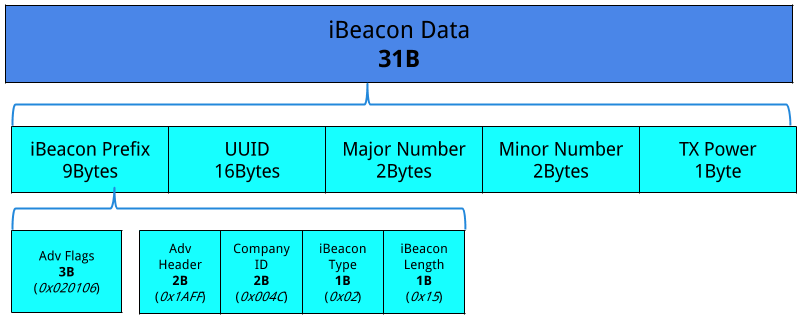
\includegraphics[width=15cm, height=8cm]{tipos_beacon_ibeacon.PNG}
            \paragraph{}
           
            \item Eddystone: reado por Google y de código abierto
            \item AltBeacon
        \end{enumerate}
    \subsection{Resultados finales}
    \subsection{Planificación}
        \paragraph{}
        Para sintetizar el proceso de desarrollo del proyecto técnico se empleará un diagrama GANTT: 
        \paragraph{}
        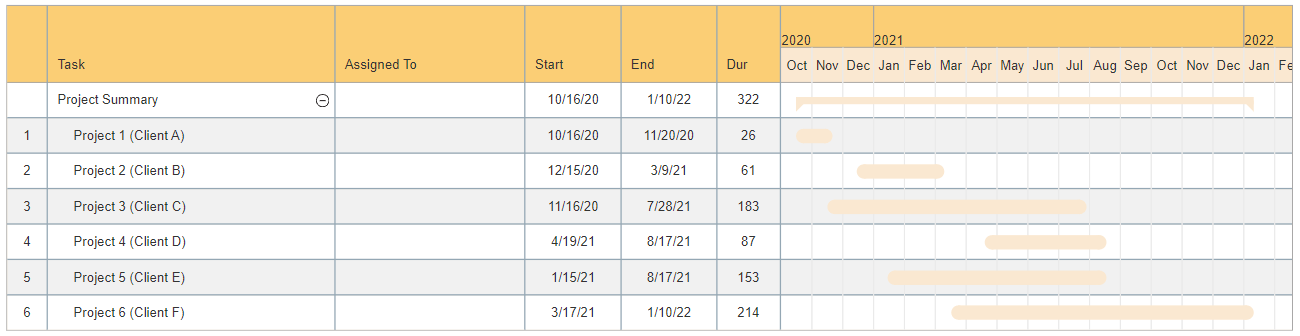
\includegraphics[width=15cm, height=8cm]{gantt.PNG}
        Fase 1: Analisis de la problemática y búsqueda de soluciones
        Fase 2: Prototipos y programación
        Fase 3: Pruebas de campo
        Fase 4: Evolución del equipo en instalación y depuración 
\section{Memoria justificativa}
    \subsection{Calculos justificactivos de la instalación}
        Calculos de consumos de los equipos y dimensionamiento de la batería.
        Los datos de partida son el consumo medio y duración del batería durante 2 años.
        \subsubsection{ Cálculo de distancia por RSSI}
            \paragraph{}
            El RSSI (Received signal strength indicator) es un indicador de la energía o potencia recibida en un mensaje de radio, 
            está asociado con la atenuación de la señal, cuanto más pequeña es su valor menor atenuación.Este valor está 
            presente no solo en Bluetooth sino también en el Wifi (2,4 GHz)o en las bandas de radio industriales, científicas y médicas,
            las denominadas ISM (desde 433MHz a 458.5MHz y desde 860MHz a 960MHz)
            \paragraph{}
            De las muestras obtenidas se puede concluir que se puede llegar a estimar la distancia a partir de los valores
            de rrsi con un error que disminuye cuanto más alejados son los elementos a medir. 
            \paragraph{}
            Los rangos del RRSI se obtiene bien por aproximaciones teóricas o bien por experimentación, esto es debido a que 
            es fuertemente alterado por las condiciones del medio en el que se encuentre. Es importante mencionar también que
            este parámetro es medido a través de un hardware que rara vez tiene un comportamiento idéntico.
            \paragraph{}
            Los modelos de cálculo del RRSI se basan en la pérdida de señal en el espacio, como sabemos la potencia de la señal
            disminuye con el cuadrado de la distancia. Esta ecuación de Friis para la transmisión libre en el espacio espacio es 
            una fórmula teórica, existen aproximaciones obtenidas por métodos empíricos:
            \begin{equation}
                P_L(d) [dB] = P_L(d_0) [dB] + 10n*\log_{10}* \frac{ d_i }{d_0 } 
            \end{equation}
            \paragraph{}
            Siendo PL (d0)  la pérdida de propagación a 1 metro y n es una constante que depende del medio, será igual
            a 2 si se encuentra en el espacio libre sin obstáculos ni reflexiones o dispersiones de señal.
            \paragraph{}
            Para calcular este parámetro 'n' se ha de aplicar la siguiente fórmula, como podemos ver para llevar a cabo el 
            cálculo se han de tomar valores empíricos de potencias:
            \begin{equation}
                n = \frac{ P_L(d_i) - P_L(d_0) }{10n*\log_{}\frac{d_i}{d_0}}
            \end{equation}
            \paragraph{}
            Por lo tanto, y una vez obtenidos los valores de potencia a distintas distancias podemos obtener la ganacia
            de la señal recibida:
            \begin{equation}
                RRSI [dBm] = -10n*\log_{10} d+ A[dBm]
            \end{equation}
            \paragraph{}
            Disponiendo ya del valor de la constante de pérdidas, d, calculado con la ecuación (2) y los valores
            de rssi medidos desde la antena receptora a 1 metro de distancia, A, podemos obtener:
            \begin{equation}
                d= 10^\frac{-(RRSI - A) }{10n}
            \end{equation}
        \subsubsection{Cálculo de consumos energéticos}
            \begin{itemize}
                \item  Active mode: 160-260mA.  Active core, ULP coprocessor and RTC
                Wifi, Bluetooth, Radio, Peripherals
                \begin{center}
                    \begin{tabular}{||c || c ||} 
                    \hline
                    ESP32 Mode & Power consumption  \\ [0.5ex] 
                    \hline\hline
                    Wi-Fi Tx packet 13dBm~21dBm & 160~260mA  \\ 
                    \hline
                    Wi-Fi/BT Tx packet 0dBm	 & 120mA  \\
                    \hline
                    Wi-Fi/BT Rx and listening & 80~90mA  \\
                    \hline
                \end{tabular}
                \end{center}
                \item  Sleep mode: 3-20mA Active core, ULP coprocessor and RTC
                Inactive: Wifi, Bluetooth, Radio, Peripherals
                \item  Light sleep mode: the CPU is paused by powering off its clock 
                pulses, while RTC and ULP-coprocessor are kept active. This results in 
                less power consumption than in modem sleep mode which is around 0.8mA.
            
                \item Deep sleep mode, the CPU, most of the RAM and all the digital 
                peripherals are powered off. The only parts of the chip that remains 
                powered on are: RTC controller, RTC peripherals (including ULP 
                co-processor), and RTC memories (slow and fast).
                The chip consumes around 0.15 mA(if ULP co-processor is powered on) to 10µA.
            
                In Deep sleep mode, power is shut off to the entire chip except RTC module. So, any data that is not in the RTC recovery memory is lost, and the chip will thus restart with a reset. This means program execution starts from the beginning once again.
            
                \item Hibernation mode: Unlike deep sleep mode, in hibernation mode the chip disables internal 8MHz oscillator and ULP-coprocessor as well. The RTC recovery memory is also powered down, meaning there’s no way we can preserve any data during hibernation mode.
            
                Everything else is shut off except only one RTC timer on the slow clock and some RTC GPIOs are active. They are responsible for waking up the chip from the hibernation mode.
                
                This reduces power consumption even further. The chip consumes around 2.5µA only in hibernation mode.
            
                \begin{center}
                    \begin{tabular}{||c | c ||} 
                    \hline
                    ESP32 Mode & Power consumption  \\ [0.5ex] 
                    \hline\hline
                    Wi-Fi Tx packet 13dBm~21dBm & 160~260mA  \\ 
                    \hline
                    Wi-Fi/BT Tx packet 0dBm	 & 120mA  \\
                    \hline
                    Wi-Fi/BT Rx and listening & 80~90mA  \\
                    \hline
                \end{tabular}
                \end{center}
            \end{itemize}
            \begin{enumerate}
                \item  yas
            \end{enumerate}


\section{Planos}
    \subsection{Plano de mecánicos}
    \subsection{Plano de eléctricos}
        \subsubsection{Esquemático del emisor beacon}
        \subsubsection{PCB circuito del emisor beacon}
        \subsubsection{Esquemático del receptor ESP32}
        \subsubsection{PCB circuito del receptor ESP32}
\section{Pliego de condiciones}
    \subsection{Prescripciones ténicas generales}
        \subsubsection{Normativa relativa a radiofrecuencia}
        \subsubsection{Normativa relativa a }
    \subsection{Prescripciones ténicas particulares}
        \subsubsection{Condiciones que ha de reunir el material}
        \subsubsection{Ejecución del proyecto}
        Placa ha de cumplir solo 1 capa
\section{Presupuestos}
    \subsection{Precios unitarios}
        \begin{center}
            \begin{tabular}{||c | c ||} 
            \hline
            ESP32 Mode & Power consumption  \\ [0.5ex] 
            \hline\hline
            Wi-Fi Tx packet 13dBm~21dBm & 160~260mA  \\ 
            \hline
            \end{tabular}
        \end{center}
    \subsection{Presupuestos Parciales}
        \subsubsection{Capitulo 1: Placa de circuito impreso emisor}
        \subsubsection{Capitulo 2: Placa de circuito impreso receptor}
        \subsubsection{Capitulo 1: }
        \subsubsection{Capitulo 1: }
    \subsection{Presupuestos Total}
        con iva
    \subsection{Factores económicos y financieros}
    Estudio de viabilidad económica
        \subsubsection{Tasa de interés de retorno(TIR)}
        \subsubsection{Valor Actual Neto (VAN)}

\section{Estudio de compativilidad electromagnética}
\subsection{test}
\subsubsection{test}

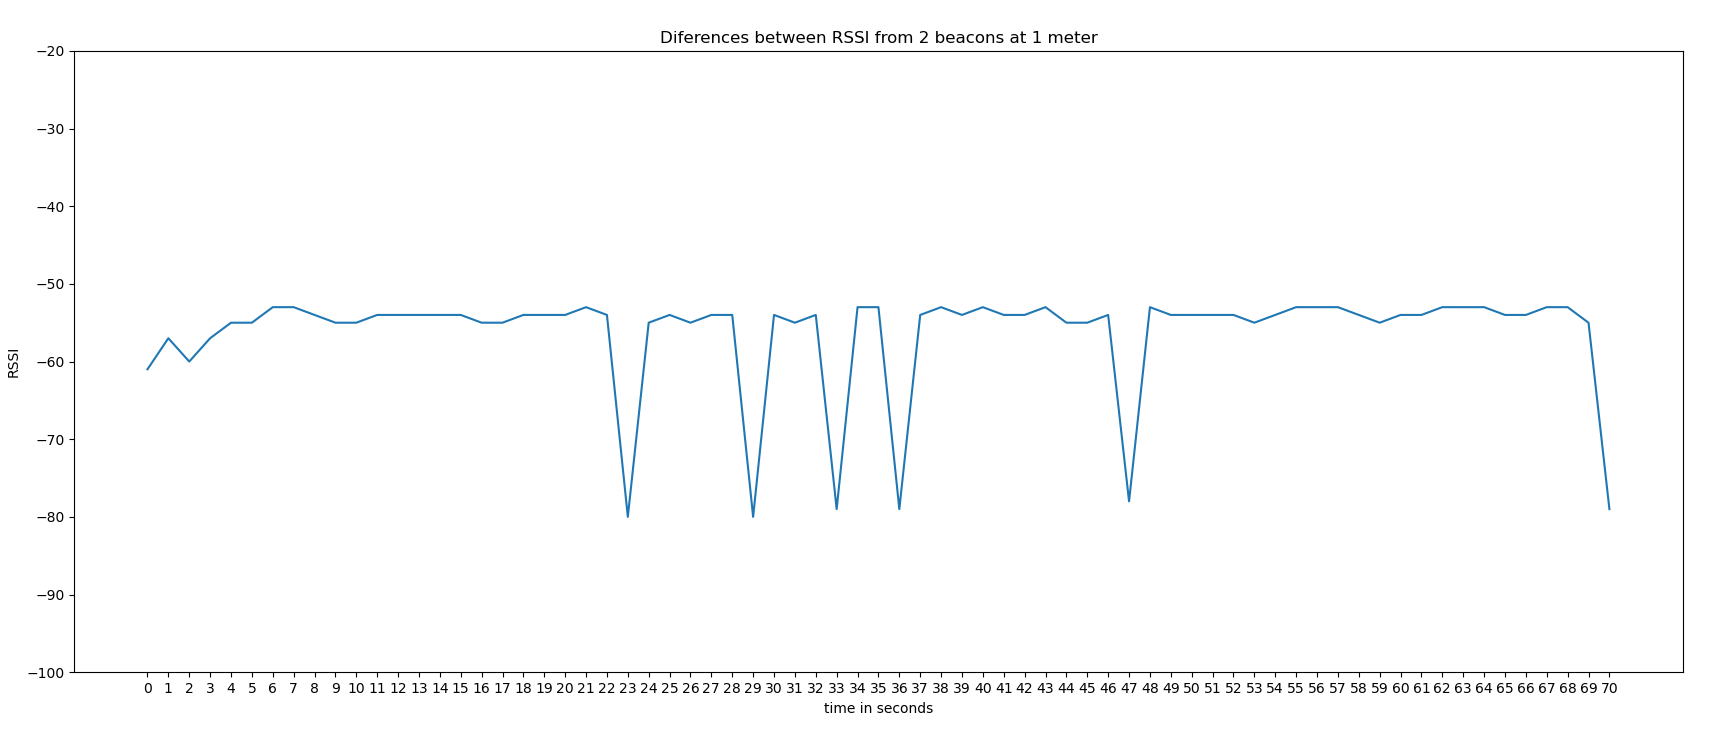
\includegraphics[scale=0.3]{5min_beacon_rssi}
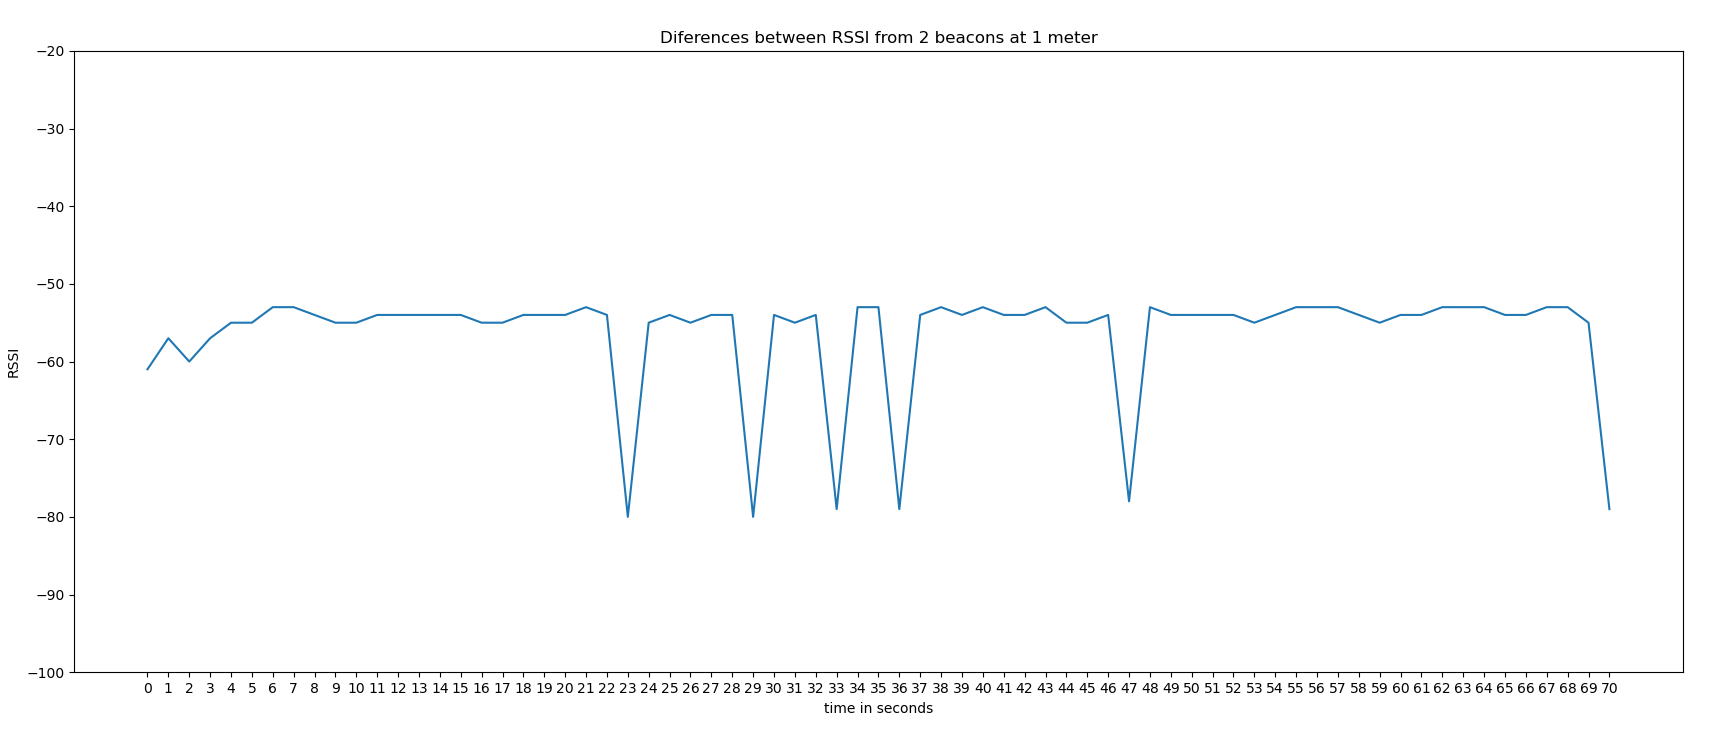
\includegraphics[width=15cm, height=8cm]{5min_beacon_rssi}
\paragraph{hola}
asdfasd



\section{Bibliografía}
\href{https://campus.masterd.es/campusvirtual/index.htm}{Something Linky} 





\end{document}